\documentclass[12pt]{article}

%--------Packages--------
\usepackage{tikz}
\usepackage{tikz-cd}
\usepackage{relsize}
\usepackage{tikz-3dplot}
\usetikzlibrary{matrix,positioning,fit}
\usetikzlibrary{calc, arrows, automata, positioning}
\usetikzlibrary{shapes}
\usetikzlibrary{patterns,hobby}
\usetikzlibrary{positioning}
\tikzset{>=latex} % for LaTeX arrow head
\colorlet{myred}{red!85!black}
\colorlet{myblue}{blue!80!black}
\colorlet{mydarkred}{myred!80!black}
\colorlet{mydarkblue}{myblue!60!black}
\tikzstyle{xline}=[myblue,thick]
\def\tick#1#2{\draw[thick] (#1) ++ (#2:0.09) --++ (#2-180:0.18)}
\tikzstyle{myarr}=[myblue!50,-{Latex[length=3,width=2]}]
\def\Nr{100}
\tikzset{fontscale/.style = {font=\relsize{#1}}}
\usepackage{esvect} %graphics for volume elem
\usepackage{booktabs}
\usepackage{tabularx}
\usepackage{multirow}
\usepackage{longtable}
\usepackage{makecell}
\usepackage{amsmath,amsfonts,amsthm,amssymb,mathrsfs,bbm,mathtools,nicefrac,witharrows,commath,cancel}
\usepackage{xargs}
\usepackage{xcolor}
\usepackage{enumitem}
\usepackage[hidelinks]{hyperref}
\usepackage[noabbrev,capitalize]{cleveref}
\usepackage[italic]{derivative}
\usepackage{xparse}
\usepackage{upgreek}
\usepackage{setspace}
\usepackage[most]{tcolorbox}
\usepackage[parfill]{parskip}
\usepackage{centernot}
\usepackage{needspace}
\usepackage{varwidth}
%\usepackage{physics}

%\renewcommand{\vec}[1]{\overrightarrow{#1}}


%--------Graphics/Images--------
\usepackage{graphicx}
\usepackage{float}
\usepackage[centerlast,small,sc]{caption}
\usepackage{subcaption} % causes weird error with \setlength{\captionmargin}{20pt}

\usepackage{pgfplots}
\pgfplotsset{compat=1.6}
\usepgfplotslibrary{fillbetween}
\usetikzlibrary{patterns}
\usepackage[outline]{contour} % glow around text
\contourlength{1.0pt}


%--------Theorem Environments--------
\newtheorem{thm}{Theorem}
\newtheorem{cor}[thm]{Corollary}
\newtheorem{lem}[thm]{Lemma}
\newtheorem{fct}[thm]{Fact}
\newtheorem{ntn}[thm]{Notation}

\theoremstyle{definition}
\newtheorem{defn}[thm]{Definition}

%\numberwithin{equation}{chapter}

\newcounter{exs}

\Crefname{thm}{Theorem}{Theorems}

\tcbuselibrary{theorems}

\newtcbtheorem
  [use counter*=thm,crefname={Example}{Examples},Crefname={Example}{Examples}]%
  {ex}
  {Example}
  {%
    before skip=10pt,after skip=10pt,
    left=0.2cm,right=0.2cm,top=0cm,
    toptitle=0.2cm,bottomtitle=0cm,
    breakable,
    toprule at break=0.2cm,
    sharp corners,
    colback=blue!10,
    coltitle=black,
    colframe=blue!10,
    fonttitle=\bfseries,
    parbox=false,
    halign=justify, % use `flush left` if document is raggedright and not justified
  }% options
  {ex}% prefix

%--------Remarks-------------
\newtcbtheorem
  [use counter*=thm,crefname={Remark}{Remarks},Crefname={Remark}{Remarks}]%
  {rmk}
  {Remark}
  {%
    before skip=10pt,after skip=10pt,
    left=0.2cm,right=0.2cm,top=0cm,
    toptitle=0.2cm,bottomtitle=0cm,
    breakable,
    toprule at break=0.2cm,
    sharp corners,
    colback=green!10,
    coltitle=black,
    colframe=green!10,
    fonttitle=\bfseries,
    parbox=false,
    halign=justify,
  }% options
  {rmk}% prefix

%--------Exercises-------------
\newtcbtheorem
  [use counter*=exs,crefname={Aufgabe}{Problems},Crefname={Aufgabe}{Problems}]%
  {exc}
  {Aufgabe}
  {%
    before skip=10pt,after skip=10pt,
    left=0.2cm,right=0.2cm,top=0cm,
    toptitle=0.2cm,bottomtitle=0cm,
    breakable,
    toprule at break=0.2cm,
    sharp corners,
    colback=purple!10,
    coltitle=black,
    colframe=purple!10,
    fonttitle=\bfseries,
    parbox=false,
    halign=justify,
  }% options
  {exercise}% prefix

%--------Readings-------------
\newtcolorbox{readings}{%
    before skip=10pt,after skip=10pt,
    left=0.2cm,right=0.2cm,top=0cm,
    toptitle=0.2cm,bottomtitle=0cm,
    breakable,
    toprule at break=0.2cm,
    sharp corners,
    colback=green!30,
    coltitle=black,
    colframe=green!30,
    fonttitle=\bfseries,
    title={Readings},
    parbox=false,
    halign=justify,
}
\newtcolorbox{oreadings}{%
    before skip=10pt,after skip=10pt,
    left=0.2cm,right=0.2cm,top=0cm,
    toptitle=0.2cm,bottomtitle=0cm,
    breakable,
    toprule at break=0.2cm,
    sharp corners,
    colback=green!20,
    coltitle=black,
    colframe=green!20,
    fonttitle=\bfseries,
    title={Optional Readings},
    parbox=false,
    halign=justify,
}

%--------important theorems-------------
\newtcolorbox{thmb}{%
    before skip=10pt,after skip=10pt,
    left=0.2cm,right=0.2cm, top=0cm,
    toptitle=0cm,bottomtitle=0cm,
    breakable,
    toprule at break=0.2cm,
    sharp corners,
    colback=gray!10,
    coltitle=black,
    colframe=gray!10,
    fonttitle=\bfseries,
    title={},
    parbox=false,
    halign=justify,
}

%-------QED-at-end-of-env---

% Define a macro for changing the QED symbol at the
% end of environments. This command allows for the
% use of \qedhere to insert the QED into, e.g., 
% equations or lists. 
\newcommand{\setEnvironmentQed}[2]{
  % #1: Environment name
  % #2: QED Symbol. Must be OK in text or math mode. 
  %     Use \ensuremath, if math is desired.
  \AtBeginEnvironment{#1}{%
    \pushQED{\qed}\renewcommand{\qedsymbol}{#2}%
  }
  \AtEndEnvironment{#1}{\popQED}
}

\setEnvironmentQed{defn}{\ensuremath{\blacksquare}}
%\setEnvironmentQed{thm}{\ensuremath{\blacksquare}}

%--------Colors-------------
\definecolor{blue}{RGB}{02,106,253}
\definecolor{red}{RGB}{245,51,30}
\definecolor{green}{RGB}{96,189,69}
\definecolor{purple}{RGB}{200,0,240}
\definecolor{nice_purple}{RGB}{128, 0, 128}
\definecolor{antiquefuchsia}{rgb}{0.57, 0.36, 0.51}
\definecolor{awesome}{rgb}{1.0, 0.13, 0.32}
\definecolor{carrotorange}{rgb}{0.93, 0.57, 0.13}
\def\b{\textcolor{blue}}
\def\r{\textcolor{red}}
\def\g{\textcolor{green}}
\def\p{\textcolor{purple}}
\def\np{\textcolor{nice_purple}}
\def\af{\textcolor{antiquefuchsia}}
\def\aw{\textcolor{awesome}}
\def\co{\textcolor{carrotorange}}

%--------Margin Tags-------------
%\usepackage{marginfix}
\let\marginnote\relax
\usepackage{marginnote}
\NewDocumentCommand{\margintag}{O{0\baselineskip}m}{%
  %\checkoddpage%
  %\ifoddpage%
    {\marginnote{\footnotesize #2}[#1]}%
  %\else%
   % {\reversemarginpar\marginnote{\footnotesize #2}[#1]}%
    % {\marginnote{\footnotesize #2}[#1]}
  %\fi
  }%
% \NewDocumentCommand{\margintagt}{O{0\baselineskip}m}{\marginpar{\vspace{#1}\footnotesize #2}}
\NewDocumentCommand{\safefootnote}{om}{\footnotemark\margintag[#1]{\textsuperscript{\tiny\arabic{footnote}} \normalfont#2}}

%--------Margin Boxes-------------
\NewDocumentEnvironment{marginbox}{O{0\baselineskip}m}{\begin{marginfigure}[#1]{\textbf{#2}}\quad}{\end{marginfigure}}

%--------Equation numbers in text-------------
\makeatletter
\NewDocumentCommand{\embeq}{m}{%
  \leavevmode\hfill\refstepcounter{equation}\textup{\tagform@{\theequation}}\label{#1}%
}
\makeatother

%--------Equation numbers in algorithms-------------
\makeatletter
\NewDocumentCommand{\algeq}{m}{%
  \leavevmode\Comment*[r]{\refstepcounter{equation}\textup{\tagform@{\theequation}}\label{#1}}%
}
\makeatother

\usepackage{etoolbox}
\makeatletter
% Remove right hand margin in algorithm
\patchcmd{\@algocf@start}% <cmd>
  {-1.5em}% <search>
  {0pt}% <replace>
  {}{}% <success><failure>
\makeatother

%--------Allow page breaks in align-------------
\allowdisplaybreaks

%--------Enumerations-------------
\setlist[enumerate]{noitemsep, topsep=-6pt, leftmargin=16pt}
\setlist[itemize]{noitemsep, topsep=-6pt}

%--------Figures-------------
\usepackage{import}
\usepackage{xifthen}
\usepackage{pdfpages}
\usepackage{transparent}

\NewDocumentCommand{\incfig}{om}{%
    \IfValueTF{#1}{%
        \def\svgwidth{#1}%
    }{%
        \def\svgwidth{\columnwidth}%
    }%
    \centering\import{./figures/}{#2.pdf_tex}%
}
\newcommand{\incplt}[1]{%
  \begin{center}
    \import{./plots/output/}{#1.pgf}
  \end{center}
}

%--------Styling part-------------
\usepackage{titlesec}
\titleclass{\part}{top} % make part like a chapter
\titleformat{\part}
[display]
{\centering\normalfont}
{\vspace{3pt}\Large\smallcaps{\partname} \thepart}
{0pt}
{\vspace{1pc}\Huge\normalfont\textit}
%
\titlespacing*{\part}{0pt}{0pt}{20pt}
%

%--------Exercises-------------
\NewDocumentEnvironment{exercise}{mm}{\begin{exc}{#1}{#2}}{\par\textit{\hyperref[solution:#2]{$\triangleright$ Solution}}
\end{exc}}


\newtheorem{nexc}{}
\crefname{nexc}{Aufgabe}{Problems}
\Crefname{nexc}{Aufgabe}{Problems}

\NewDocumentCommand{\excheading}{}{\needspace{6\baselineskip}\section*{Problems}}

\NewDocumentEnvironment{nexercise}{mm}{%
  % Reserve enough space for exactly two lines (heading + one line).
  \needspace{2\baselineskip}%
  \begin{nexc}%
  \hyperref[solution:#2]{\b{\textbf{#1.}}}\label{exercise:#2}%
  % Possibly force them into the same paragraph:
  \par\nobreak
  % or \nolinebreak, if you prefer to keep them in one paragraph.
}{%
  \end{nexc}%
}

\NewDocumentCommand{\exerciseref}{mo}{\margintag{\normalfont\textbf{\Cref{exercise:#1} \IfValueT{#2}{({#2})}{}}}}
\newcommand*\circled[1]{\tikz[baseline=(char.base)]{
            \node[shape=circle,draw,inner sep=1pt] (char) {#1};}}
\NewDocumentCommand{\exerciserefmark}{mo}{\hyperref[exercise:#1]{\circled{\normalfont\textbf{?}}}\exerciseref{#1}[#2]}

%--------Solutions-------------
\NewDocumentEnvironment{tips}{m}{\paragraph{\normalfont{\textbf{Tipps zu \cref{exercise:#1}.}}}\label{solution:#1}}{}

\newcommand{\blankpage}{\newpage\hbox{}\thispagestyle{empty}\newpage}
\newcommand{\emptyparagraph}{\paragraph{}\noindent}

\newcommand{\course}{\ifthenelse{\boolean{manuscript}}{manuscript}{course}\xspace}

% Comments
\newcommand{\ak}[1]{{\bf[AK: #1]}}

%--------Basic Math--------
\NewDocumentCommand{\floor}{m}{\left\lfloor #1 \right\rfloor}
\NewDocumentCommand{\ceil}{m}{\left\lceil #1 \right\rceil}
\NewDocumentCommand{\ip}{m}{\left\langle #1 \right\rangle}

%\newcommand*{\abs}[1]{\left| #1 \right|}
\newcommand*{\card}[1]{\left| #1 \right|}
%\NewDocumentCommand{\norm}{sm}{\IfBooleanTF{#1}{\|#2\|}{\left\| #2 \right\|}}

\newcommand*{\const}{\mathrm{const}}

\newcommand*{\defeq}{\overset{.}{=}}
\newcommand*{\eqdef}{\overset{.}{=}}

\DeclareMathOperator*{\argmax}{arg\,max}
\DeclareMathOperator*{\argmin}{arg\,min}


\DeclarePairedDelimiter\parentheses{(}{)}
\DeclarePairedDelimiter\brackets{[}{]}
\DeclarePairedDelimiter\braces{\{}{\}}


%--------Sets--------
\newcommand{\R}{\mathbb{R}}
\newcommand{\Rzero}{\mathbb{R}_{\geq 0}}
\newcommand{\Nat}{\mathbb{N}}
\newcommand{\NatZ}{\mathbb{N}_0}


%--------Symbols--------
%\renewcommand{\vec}[1]{\mathbold{#1}}
%\newcommand{\mat}[1]{\mathbold{#1}}
\newcommand{\rvec}[1]{\mathbf{#1}}
%\newcommand{\set}[1]{#1}
\newcommand{\spa}[1]{\mathcal{#1}}

\newcommand{\mean}[1]{\overline{#1}}
\newcommand{\compl}[1]{\overline{#1}}
\newcommand{\old}[1]{#1^{\mathrm{old}}}
\newcommand{\opt}[1]{#1^\star}

\newcommand{\altpi}{\Pi} % \vec{\uppi}



\NewDocumentCommand{\fnv}{oo}{v\IfValueT{#2}{_{#2}}\IfValueT{#1}{^{#1}}}
\RenewDocumentCommand{\v}{somo}{\IfBooleanTF{#1}{\fnv[\star][#4]\parentheses{#3}}{\fnv[#2][#4]\parentheses{#3}}}
\NewDocumentCommand{\fnq}{oo}{q\IfValueT{#2}{_{#2}}\IfValueT{#1}{^{#1}}}
\NewDocumentCommand{\q}{sommo}{\IfBooleanTF{#1}{\fnq[\star][#5]\parentheses{#3,#4}}{\fnq[#2][#5]\parentheses{#3,#4}}}
\NewDocumentCommand{\fnV}{oo}{V\IfValueT{#2}{_{#2}}\IfValueT{#1}{^{#1}}}
\NewDocumentCommand{\V}{somo}{\IfBooleanTF{#1}{\fnV[\star][#4]\parentheses{#3}}{\fnV[#2][#4]\parentheses{#3}}}
\NewDocumentCommand{\fnQ}{oo}{Q\IfValueT{#2}{_{#2}}\IfValueT{#1}{^{#1}}}
\NewDocumentCommand{\Q}{sommo}{\IfBooleanTF{#1}{\fnQ[\star][#5]\parentheses{#3,#4}}{\fnQ[#2][#5]\parentheses{#3,#4}}}
\NewDocumentCommand{\fna}{oo}{a\IfValueT{#2}{_{#2}}\IfValueT{#1}{^{#1}}}
\RenewDocumentCommand{\a}{sommo}{\IfBooleanTF{#1}{\fna[\star][#5]\parentheses{#3,#4}}{\fna[#2][#5]\parentheses{#3,#4}}}
\NewDocumentCommand{\fnA}{oo}{A\IfValueT{#2}{_{#2}}\IfValueT{#1}{^{#1}}}
\NewDocumentCommand{\fnAhat}{oo}{\hat{A}\IfValueT{#2}{_{#2}}\IfValueT{#1}{^{#1}}}
\NewDocumentCommand{\A}{sommo}{\IfBooleanTF{#1}{\fnA[\star][#5]\parentheses{#3,#4}}{\fnA[#2][#5]\parentheses{#3,#4}}}
\NewDocumentCommand{\fnj}{o}{J\IfValueT{#1}{_{#1}}}
\RenewDocumentCommand{\j}{mo}{\fnj[#2]\parentheses{#1}}
\NewDocumentCommand{\fnJ}{o}{\widehat{J}\IfValueT{#1}{_{#1}}}
\NewDocumentCommand{\J}{mo}{\fnJ[#2]\parentheses{#1}}

\NewDocumentCommand{\pset}{m}{\mathcal{P}\parentheses*{#1}}

\NewDocumentCommand{\pf}{mm}{{#1}_\sharp #2}

\NewDocumentCommand{\grad}{e_}{\boldsymbol{\nabla}\IfValueT{#1}{_{\!\!#1}\,}}
\NewDocumentCommand{\jac}{}{\mD}
\NewDocumentCommand{\hes}{}{\mH}
\NewDocumentCommand{\dive}{}{\grad\cdot}
\NewDocumentCommand{\lapl}{}{\Delta}

\NewDocumentCommand{\BigO}{m}{O\parentheses*{#1}}
\NewDocumentCommand{\BigOTil}{m}{\widetilde{O}\parentheses*{#1}}

\NewDocumentCommand{\transpose}{m}{#1^\top}
\NewDocumentCommand{\inv}{m}{#1^{-1}}
\RenewDocumentCommand{\det}{m}{\mathrm{det}\parentheses*{#1}}
\NewDocumentCommand{\tr}{m}{\mathrm{tr}\parentheses*{#1}}
\NewDocumentCommand{\diag}{om}{\mathrm{diag}\IfValueT{#1}{_{#1}}{}\braces{#2}}
\NewDocumentCommand{\msqrt}{m}{#1^{\nicefrac{1}{2}}}
\NewDocumentCommand{\vecop}{m}{\mathrm{vec}\brackets{#1}}

%--------Common vectors/matrices/sets--------
\newcommand{\vzero}{\vec{0}}
\newcommand{\vone}{\vec{1}}
\newcommand{\va}{\vec{a}}
\newcommand{\vap}{\vec{a'}}
\newcommand{\vas}{\vec{\opt{a}}}
\newcommand{\vb}{\vec{b}}
\newcommand{\vc}{\vec{c}}
\newcommand{\vd}{\vec{d}}
\newcommand{\ve}{\vec{e}}
\newcommand{\vf}{\vec{f}}
\newcommand{\vfhat}{\vec{\hat{f}}}
\newcommand{\vg}{\vec{g}}
\newcommand{\vh}{\vec{h}}
\newcommand{\vk}{\vec{k}}
\newcommand{\vm}{\vec{m}}
\newcommand{\vp}{\vec{p}}
\newcommand{\vq}{\vec{q}}
\newcommand{\vr}{\vec{r}}
\newcommand{\vs}{\vec{s}}
\newcommand{\vt}{\vec{t}}
\newcommand{\vu}{\vec{u}}
\newcommand{\vve}{\vec{v}}
\newcommand{\vvp}{\vec{v'}}
\newcommand{\vvs}{\vec{\opt{v}}}
\newcommand{\vw}{\vec{w}}
\newcommand{\vwhat}{\vec{\hat{w}}}
\newcommand{\vx}{\vec{x}}
\newcommand{\vxp}{\vec{x'}}
\newcommand{\vxs}{\vec{\opt{x}}}
\newcommand{\vy}{\vec{y}}
\newcommand{\vyp}{\vec{y'}}
\newcommand{\vz}{\vec{z}}
\newcommand{\valpha}{\vec{\alpha}}
\newcommand{\valphahat}{\vec{\hat{\alpha}}}
\newcommand{\vdelta}{\vec{\delta}}
\newcommand{\vDelta}{\vec{\Delta}}
\newcommand{\vepsilon}{\vec{\epsilon}}
\newcommand{\vvarepsilon}{\vec{\varepsilon}}
\newcommand{\veta}{\vec{\eta}}
\newcommand{\vlambda}{\vec{\lambda}}
\newcommand{\vmu}{\vec{\mu}}
\newcommand{\vmuhat}{\vec{\hat{\mu}}}
\newcommand{\vmup}{\vec{\mu'}}
\newcommand{\vnu}{\vec{\nu}}
\newcommand{\vomega}{\vec{\omega}}
\newcommand{\vphi}{\vec{\phi}}
\newcommand{\vpi}{\vec{\pi}}
\newcommand{\vpsi}{\vec{\psi}}
\newcommand{\vvarphi}{\vec{\varphi}}
\newcommand{\vvarphihat}{\vec{\hat{\varphi}}}
\newcommand{\vtheta}{\vec{\theta}}
\newcommand{\vthetahat}{\vec{\hat{\theta}}}
\newcommand{\vxi}{\vec{\xi}}
\newcommand{\mzero}{\mat{0}}
\newcommand{\mA}{\mat{A}}
\newcommand{\mB}{\mat{B}}
\newcommand{\mBs}{\mat{\opt{B}}}
\newcommand{\mC}{\mat{C}}
\newcommand{\mD}{\mat{D}}
\newcommand{\mF}{\mat{F}}
\newcommand{\mH}{\mat{H}}
\newcommand{\mI}{\mat{I}}
\newcommand{\mK}{\mat{K}}
\newcommand{\mL}{\mat{L}}
\newcommand{\mCalL}{\mat{\mathcal{L}}}
\newcommand{\mM}{\mat{M}}
\newcommand{\mP}{\mat{P}}
\newcommand{\mQ}{\mat{Q}}
\newcommand{\mS}{\mat{S}}
\newcommand{\mT}{\mat{T}}
\newcommand{\mU}{\mat{U}}
\newcommand{\mV}{\mat{V}}
\newcommand{\mW}{\mat{W}}
\newcommand{\mX}{\mat{X}}
\newcommand{\mLambda}{\mat{\Lambda}}
\newcommand{\mPhi}{\mat{\Phi}}
\newcommand{\mPi}{\mat{\Pi}}
\newcommand{\mSigma}{\mat{\Sigma}}
\newcommand{\mSigmap}{\mat{\Sigma'}}
\newcommand{\rG}{\rvec{G}}
\newcommand{\rQ}{\rvec{Q}}
\newcommand{\rU}{\rvec{U}}
\newcommand{\rV}{\rvec{V}}
\newcommand{\rW}{\rvec{W}}
\newcommand{\rX}{\rvec{X}}
\newcommand{\rXp}{\rvec{X'}}
\newcommand{\rY}{\rvec{Y}}
\newcommand{\rZ}{\rvec{Z}}
\newcommand{\sA}{\set{A}}
\newcommand{\sB}{\set{B}}
\newcommand{\sC}{\set{C}}
\newcommand{\sD}{\set{D}}
\newcommand{\sI}{\set{I}}
\newcommand{\sM}{\set{M}}
\newcommand{\sS}{\set{S}}
\newcommand{\sU}{\set{U}}
\newcommand{\sX}{\set{X}}
\newcommand{\sY}{\set{Y}}
\newcommand{\sZ}{\set{Z}}
\newcommand{\spA}{\spa{A}}
\newcommand{\spB}{\spa{B}}
\newcommand{\spC}{\spa{C}}
\newcommand{\spD}{\spa{D}}
\newcommand{\spF}{\spa{F}}
\newcommand{\spH}{\spa{H}}
\newcommand{\spL}{\spa{L}}
\newcommand{\spM}{\spa{M}}
\newcommand{\spO}{\spa{O}}
\newcommand{\spP}{\spa{P}}
\newcommand{\spQ}{\spa{Q}}
\newcommand{\spT}{\spa{T}}
\newcommand{\spW}{\spa{W}}
\newcommand{\spX}{\spa{X}}
\newcommand{\spY}{\spa{Y}}
\newcommand{\spZ}{\spa{Z}}
\newcommand{\fs}{\opt{f}}
\newcommand{\ps}{\opt{p}}
\newcommand{\qs}{\opt{q}}
\newcommand{\xs}{\opt{x}}
\newcommand{\ys}{\opt{y}}
\newcommand{\Bs}{\opt{B}}
\newcommand{\Qs}{\opt{Q}}
\newcommand{\sSs}{\opt{\sS}}
\newcommand{\hQs}{\opt{\hat{Q}}}
\newcommand{\Vs}{\opt{V}}
\newcommand{\pis}{\opt{\pi}}

\newcommand{\vF}{\rvec{F}}
\newcommand{\vS}{\rvec{S}}
\newcommand{\vT}{\rvec{T}}


\renewcommand\qedsymbol{$\blacksquare$}


\newcommand{\dx}{\mathrm{d}x}
\newcommand{\ddx}{\frac{\mathrm{d}}{\mathrm{d}x}}
\newcommand{\dt}{\mathrm{d}t}
\newcommand{\du}{\mathrm{d}u}
\newcommand{\dve}{\mathrm{d}v}
\newcommand{\dw}{\mathrm{d}w}
\newcommand{\dy}{\mathrm{d}y}
\newcommand{\dz}{\mathrm{d}z}
\newcommand{\dF}{\mathrm{d}F}
\newcommand{\dV}{\mathrm{d}V}
\newcommand{\dr}{\mathrm{d}r}
\newcommand{\dtheta}{\mathrm{d}\theta}
\newcommand{\drho}{\mathrm{d}\rho}
\newcommand{\dphi}{\mathrm{d}\varphi}

\newcommand{\Rn}{\mathbb{R}^n}
\newcommand{\Rm}{\mathbb{R}^m}
\newcommand{\Rk}{\mathbb{R}^k}
\newcommand{\und}{\text{ und }}
\newcommand{\oder}{\text{ oder }}
\newcommand{\bydef}{\underset{def.}{=}}
\newcommand{\BH}{\underset{\textrm{B-H}}{=}}

\newcommand{\Follows}{\Longrightarrow\ }
\newcommand{\sameas}{\Longleftrightarrow}
\newcommandx{\Laplace}[2][1=f(t), 2=s]{\mathscr{L}\{#1\}(#2)}
\newcommandx{\LaplaceInv}[2][1=F(s), 2=t]{\mathscr{L}^{-1}\{#1\}(#2)}
\DeclareMathOperator{\arccosh}{Arcosh}
\DeclareMathOperator{\arcsinh}{Arsinh}
\DeclareMathOperator{\arctanh}{Artanh}
\DeclareMathOperator{\arcsech}{arcsech}
\DeclareMathOperator{\arccsch}{arcCsch}
\DeclareMathOperator{\arccoth}{arcCoth} 

\def\doubleunderline#1{\underline{\underline{#1}}}
\def\ez{\begin{flushright}\underline{ez.}\end{flushright}}
%\[
%   \Laplace[\cos(x)]=\int_{t=0}^{\infty}f(t)e^{-st}dt
%\]

\newcommand{\Z}{\mathbb{Z}}
\newcommand{\N}{\mathbb{N}}

\newcommand{\C}{\mathbb{C}}

\newcommand{\inttext}{\shortintertext}

% The following example defines \colorboxed as wrapper around amsmath's \boxed to set the frame color. It uses package xcolor for the color support to save the current color . before changing the color for the frame. Inside the box, the previous saved color is restored. This avoids a white background of \fcolorbox, since there is no "transparent" color.

% The macro also supports an optional argument for specifying the color model.

% Definition of \boxed in amsmath.sty:
% \newcommand{\boxed}[1]{\fbox{\m@th$\displaystyle#1$}}


% Syntax: \colorboxed[<color model>]{<color specification>}{<math formula>}
\newcommand*{\colorboxed}{}
\def\colorboxed#1#{%
  \colorboxedAux{#1}%
}
\newcommand*{\colorboxedAux}[3]{%
  % #1: optional argument for color model
  % #2: color specification
  % #3: formula
  \begingroup
    \colorlet{cb@saved}{.}%
    \color#1{#2}%
    \boxed{%
      \color{cb@saved}%
      #3%
    }%
  \endgroup
}

%
\usepackage[utf8]{inputenc}
\usepackage[ngerman]{babel}
\usepackage[a4paper, top=1in, bottom=1.3in, rmargin=1.5in, left=1.4in, marginparwidth=80pt]{geometry}
\usepackage{etoc}
\usepackage{csquotes}
%\usepackage{emoji}
%\usepackage[tight]{minitoc}


\begin{document}
\title{\vspace*{-2.5em}Problem Set 4, Summary \& Tips}
\author{Vikram R. Damani\\
    Analysis~II}

\maketitle
%\dosectoc
%\sectoc

%\tableofcontents % //FIXME: make small toc

\section{Tipps}

\begin{nexercise}{Aufgabe 1}{1}\addcontentsline{toc}{subsection}{A1}
\end{nexercise}

\begin{tips}{1}
    lol
\end{tips}\vspace*{1em}

\begin{nexercise}{Aufgabe 2}{2}
    d
\end{nexercise}

\begin{tips}{2}
    d
\end{tips}\vspace*{1em}

\begin{nexercise}{Aufgabe 3}{3}
    dooooooooooooooooo o ooo oo o ooo oooo ooooo oo oo oo oooo o o o o o o o o oo oooooooooooooooooooooooooooooooooooooo o oo oo oo oooo oooo o oo o o o o o  o o o ooooooooooooooooooooooooooooooooooooooooooooooooooooooooooooooooooooooooooooooooooooooooooooooooooooo
\end{nexercise}

\begin{tips}{3}
    daaaaaaaaaaaaaaaaaaaaaaaaaaaaaaaaaa a a a a a a  a a a  a a  a  a a  a a aaaaaaaaaaaaaaaaaaaaaaaaaaaaaaaaaaaaaaaaaaaaaaaaaa aaa  a a  a a  a a  a a a a a a a a a
\end{tips}

\section{Theorie}
%\localtableofcontents

% \begin{displayquote}
%     \emph{Fuck it, there's not much to say}
% \end{displayquote}
% \begin{flushright}
%     Kottas, \today.
% \end{flushright}

% \begin{displayquote}
%     \emph{Yeah, but he's dead}
% \end{displayquote}
% \begin{flushright}
%     Kottas, \today.
% \end{flushright}

% \begin{displayquote}
%     \emph{Yeah, ants dont do taxes, do they\dots}
% \end{displayquote}
% \begin{flushright}
%     Kottas, \today.
% \end{flushright}

\begin{thmb}{\np{\emph{[Satz von \emph{Leibnitz} (Parameter in Integralgrenzen)].}}} Sei
    \begin{align}
        \Psi(x)\defeq\int_{u(x)}^{v(x)}f(x,t)\dt.
    \end{align}
    Dann ist die Ableitung
    \begin{align}
        \Psi'(x) & =\ddx \int_{u(x)}^{v(x)} f(t,x)\dt                                                                                       \\[5pt]
                 & =\colorboxed{antiquefuchsia}{\int_{u(x)}^{v(x)}\pdv{}{x}f(x,t)\dt + f(x,\r{v(x)})\,\r{v'(x)} - f(x,\r{u(x)})\,\r{u'(x)}}
    \end{align}

    \b{\emph{Spezialfälle}}:
    \begin{enumerate}[label=(\alph*)]
        \item $u(x)=a, \,v(x)=b\;\;\;\const.\implies u'=v'=0$ und es gilt also
              \begin{align}
                  \Psi'(x) =\colorboxed{antiquefuchsia}{\int_{a}^{b}\pdv{}{x}f(x,t)\dt}
              \end{align}
        \item $u(x)=a\;\const.\text{ und } \,v(x)=x,\text{ sowie }f(x,t)=g(t)$ unabh.\ von $x$ $\implies u'=0,\;g_x\equiv0,\;v'=1$ und es gilt also
              \begin{align}
                  \ddx\int_{0}^{x}g(t)\dt=g(x),
              \end{align}
              der Hauptsatz der Infinitesimalrechnung.
    \end{enumerate}
\end{thmb}\vspace*{1em}

\subsection{Vektorfelder}

\begin{defn}{\b{[Vektorfelder].}} Ein Vektorfeld weist jedem Punkt im Raum einen Vektor der gleichen Dimension zu.

    \textbf{Beispiele:}
    \begin{enumerate}[label=(\roman*)]
        \item Magnet/Elektrisches Feld
        \item Wind/Strömung
        \item Wärmefluss
              %\item Anything is a vectorfield if you're brave enough % including your mom
    \end{enumerate}
\end{defn}

\begin{figure}[htbp!]
    \centering
    \begin{tikzpicture}[>=latex, x=1.5cm, y=1.5cm, scale=1.5, font=\footnotesize]
        \def\length{sqrt(1+(x+y)^2)}
        \begin{axis}[
                axis lines=middle,
                view={0}{90},
                domain=-2.5:2.5,
                samples=18,
                axis equal image,
                ticklabel style={font=\tiny}
            ]
            \addplot3[
                blue!40!red,
                quiver={u={1/(\length)},
                        v={(x+y)/(\length)},
                        scale arrows=0.2,
                        every arrow/.append style={-latex}},
            ] (x,y,0);
        \end{axis}
    \end{tikzpicture}
\end{figure}

\begin{defn}{\b{[Skalarfeld]}} Sei $\mathbf{B}\subseteq\R^3$. Eine Funktion
    \begin{align}
        f\colon\quad \mathbf{B} & \longrightarrow\R    \\
        (x,y,z)                 & \longmapsto f(x,y,z)
    \end{align}
    in 3 Variablen ist ein Skalarfeld.
\end{defn}\vspace*{1em}

\begin{defn}{\b{[Vektorfeld]}} Ein Vektorfeld ist eine Funktion
    \begin{align}
        f\colon\quad \mathbf{B} & \longrightarrow\R^3                                \\
        \vec{r}                 & \longmapsto \vec{v}\,(\vec{r}\,)=\begin{pmatrix}
                                                                       v_1(x,y,z) \\[3pt]
                                                                       v_2(x,y,z) \\[3pt]
                                                                       v_3(x,y,z)
                                                                   \end{pmatrix}
    \end{align}
    \begin{rmk}{}{}
        Falls  $\mathbf{B}\subseteq\R^2$ und $\vec{v}: \mathbf{B}\to\R^2$, ist $\vec{v}$ ein \emph{ebenes Vektorfeld}.
    \end{rmk}
    \begin{rmk}{}{}
        Manche Vektorfelder sind ausserdem zeitabhänging, d.h.\ $\vve\,(\vr,t)\in\R^3$. Diese Vektorfelder nennt man instationär.
    \end{rmk}
\end{defn}\vspace*{1em}

\begin{defn}{\b{[Feldlinien]}}
    Eine Kurve $K\subset{B}$, die an jedem Punkt tangential zum Vektorfeld $\vve\,(\vr\,)$ ist, heisst Feldlinie von $\vve$.
\end{defn}\vspace*{1em}

\begin{defn}{\b{[Homogenes Vektorfeld]}} Ein konstantes Vektorfeld $\vve\,(\vr\,)=\va$ heisst homogen.
\end{defn}

\colorlet{Ecolor}{orange!90!black}
\colorlet{pluscolor}{red!60!black}
\colorlet{minuscolor}{blue!60!black}
\tikzstyle{anode}=[top color=red!20, bottom color=red!50]
\tikzstyle{cathode}=[top color=blue!20, bottom color=blue!40]
\tikzstyle{charge+}=[very thin,top color=red!50, bottom color=red!80]
\tikzstyle{charge-}=[very thin,top color=blue!40, bottom color=blue!70]
\tikzset{EFieldLine/.style={
            Ecolor, decoration={markings, mark=at position #1 with {\arrow{stealth}}}, postaction={decorate}}
}

\def\dph{0.3} % dipole height
\def\dpw{0.1} % dipole width
\def\dipole#1{
    \begin{scope}[shift={(#1)}]
        \draw[charge-] (-\dph,0) to[out=90,in=180] (0,\dpw) -- (0,-\dpw) to[out=180,in=-90] cycle;
        \draw[charge+] ( \dph,0) to[out=90,in=0] (0,\dpw) -- (0,-\dpw) to[out=  0,in=-90] cycle;
        \node[scale=0.7] at (-\dph/2,0) {$-$};
        \node[scale=0.7] at ( \dph/2,0) {$+$};
    \end{scope}
}

\def\height{5}
\def\width{3}
\def\platewidth{0.5}
\def\dielwidth{0.13*\width}
\def\nfieldlines{20}
\def\ncharges{7}

% capacitor with dipolar polarization
\begin{figure}[htbp!]
    \centering
    \begin{tikzpicture}

        % dielectric slab
        \draw[orange!60!black,fill=orange!80!brown!5]
        (\dielwidth,-0.03*\height) rectangle (\width-\dielwidth,1.03*\height)
        node[Ecolor, above=3cm, midway] {$\vec E$}
        node[above, pluscolor] {$+Q_\text{surf}$}
        node[above, minuscolor] at (1.3*\dielwidth,1.03*\height) {$-Q_\text{surf}$};

        % electric field
        \foreach \i [evaluate={\y=(\i-0.75)*\height/(\nfieldlines-0.5);}] in {1,...,\nfieldlines}{
                \draw[EFieldLine={0.54},very thick] (0,\y) --++ (\width,0);
            }

        % plates
        \draw[anode] (0,0) rectangle++ (-\platewidth,\height)
        node[left, pluscolor] {$+Q_\text{C}$};
        \draw[cathode] (\width,0) rectangle++ (\platewidth,\height)
        node[right, minuscolor] {$-Q_\text{C}$};
    \end{tikzpicture}
    \caption{Homogenes Vektorfeld eines Plattenkondensators.}
\end{figure}

\begin{defn}{\b{[Rotationsfeld]}} Bezeichnet $\vec{\omega}=\begin{pmatrix}
            \omega_1 & \omega_2 & \omega_3
        \end{pmatrix}\in\R^3$ ($\const.$) eine Winkelgeschwindigkeit um die Drehachse $\vec{\omega}$,
    so ist
    \begin{align}
        \vve\,(\vr\,)=\vec{\omega}\times\vr=\begin{pmatrix}
                                                \omega_2 z -\omega_3 y \\
                                                \omega_3 x-\omega_1 z  \\
                                                \omega_1 y-\omega_2 y
                                            \end{pmatrix}
    \end{align}
\end{defn}

\subsection{Differentialoperatoren}

\begin{defn}{\b{[Gradientenfeld]}}
    Sei $f$ ein Skalarfeld. Dann ist
    \begin{align}
        grad(f)=\grad{f(\vr\,)}=\begin{pmatrix}
                                    \pdv{f}{x} \\[4pt]
                                    \pdv{f}{y} \\[4pt]
                                    \pdv{f}{z}
                                \end{pmatrix}\in\R^3
    \end{align} das zugehörige Gradientenfeld.
\end{defn}

\begin{rmk}{}{} Zuweisungen die Funktionen in andere Funktionen umwandeln (Funktion~$\mapsto$~Funktion) nennt man Operatoren.
\end{rmk}\vspace*{1em}

\begin{defn}{\b{[Divergenz]}} Für ein Vektorfeld $\vve$ ist der Divergenzoperator wie folgt definiert
    \begin{align}
        \mathrm{div}(\vve)=\nabla\cdot{\vve}=(v_1)_x+(v_2)_y+(v_2)_z=f(x,y,z)
    \end{align} ein Skalarfeld.
\end{defn}

\begin{rmk}{}{}
Der Laplace Operator kann auch als Divergenz des Gradientenfeldes geschrieben werden, also
\begin{align}
    \Delta{f}=\nabla\cdot\grad{f}=(f_x)_x+(f_y)_y+(f_z)_z
\end{align}
\end{rmk}

\begin{defn}{\b{[Rotation]}} Sei $\vve$ ein Vektorfeld. Dann ist
    \begin{align}
        \mathrm{rot}(\vve)=\vec\nabla\times\vve=\begin{pmatrix}
            v_{3,y}-v_{2,z}\\
            v_{1,z}-v_{3,x}\\
            v_{2,x}-v_{1,y}
        \end{pmatrix}
    \end{align}
\end{defn}

Es gilt also
\begin{figure}[htbp!]
    \centering
    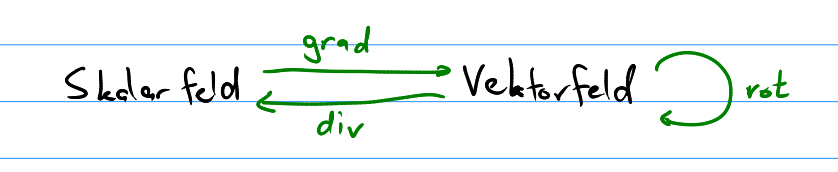
\includegraphics[scale=0.6]{imgs/skalarfeld-vektorfeld-relation.png}
\end{figure}

\end{document}

\begin{defn}{Funktionen in mehreren Variablen}
    Eine Funktion $f: D \to \R$ mit $D \subseteq \R^n$ ist eine Abbildung, die jedem $x \in D$ genau ein $f(x) \in \R$ zuordnet.
\end{defn}

\begin{tikzpicture}

    \begin{axis}[
            %axis background/.style={fill=green!10},
            %3d box=complete*,
            grid=major,
            %colorbar % show key
        ]
        \addplot3[surf] {{sin(deg(x)) * y*(1-y)}};
    \end{axis}

\end{tikzpicture}

